\documentclass[aspectratio=169]{beamer}
\usetheme{vub} % This will automatically load all fonts (Roboto and TeX Gyre Adventor
% for titles), and the VUB colors. Also includes the triangle.
\usepackage{graphicx}
\usepackage{tikz}

\title{Flick.rs}
\subtitle{Creating Hogwarts' Flickr without magic} % Can be omitted
\author{Ruben De Smet, Thibaut Vandervelden, Tom Godden}
\date{January 15, 2021}

\AtBeginPart{\frame{\partpage}}
\AtBeginSection{\frame{\sectionpage}}
\AtBeginSubsection{\frame{\subsectionpage}}

\begin{document}
\frame{\maketitle} % Automatic titlepage with VUB logo.

\begin{frame}
  \begin{tikzpicture}[
      planet/.style = {circle, draw=none, fill=blue!30,
        font=\large\bfseries,
        text width=24mm, inner sep=1mm,align=center}, %<---
      satellite/.style = {circle, draw=none, fill=####1!30,
        text width=23mm, inner sep=1mm, align=center},%<---
  ]
    % planet
    \node[inner sep=1mm,align=center] (p) at (0,0) {
      
\includegraphics[width=.4\textwidth]{logo.png}
    };
    \node (s1) [satellite=orange] at (35:5.4) {peer-to-peer};
    \node (s2) [satellite=orange] at (0:5.4) {private};
    \node (s3) [satellite=orange] at (-35:5.4) {social network};
    \node(ref) at (9,-4.4){De Smet \textit{et al.}, 2018};
    \pause
    \draw[radius=2cm, draw=none, fill=red!30, align=center] (9.4,0) circle node {
      \textbf{access control:}\\
      large ACLs
    };
  \end{tikzpicture}
\end{frame}

\section{attribute based encryption}

\begin{frame}
	\begin{tikzpicture}
	\node[inner sep=1mm,align=center] at (0,0) {
    
\includegraphics[width=.25\textwidth]{harry.png}
  };
	\pause
	\node[inner sep=1mm,align=center] at (5,0) {
    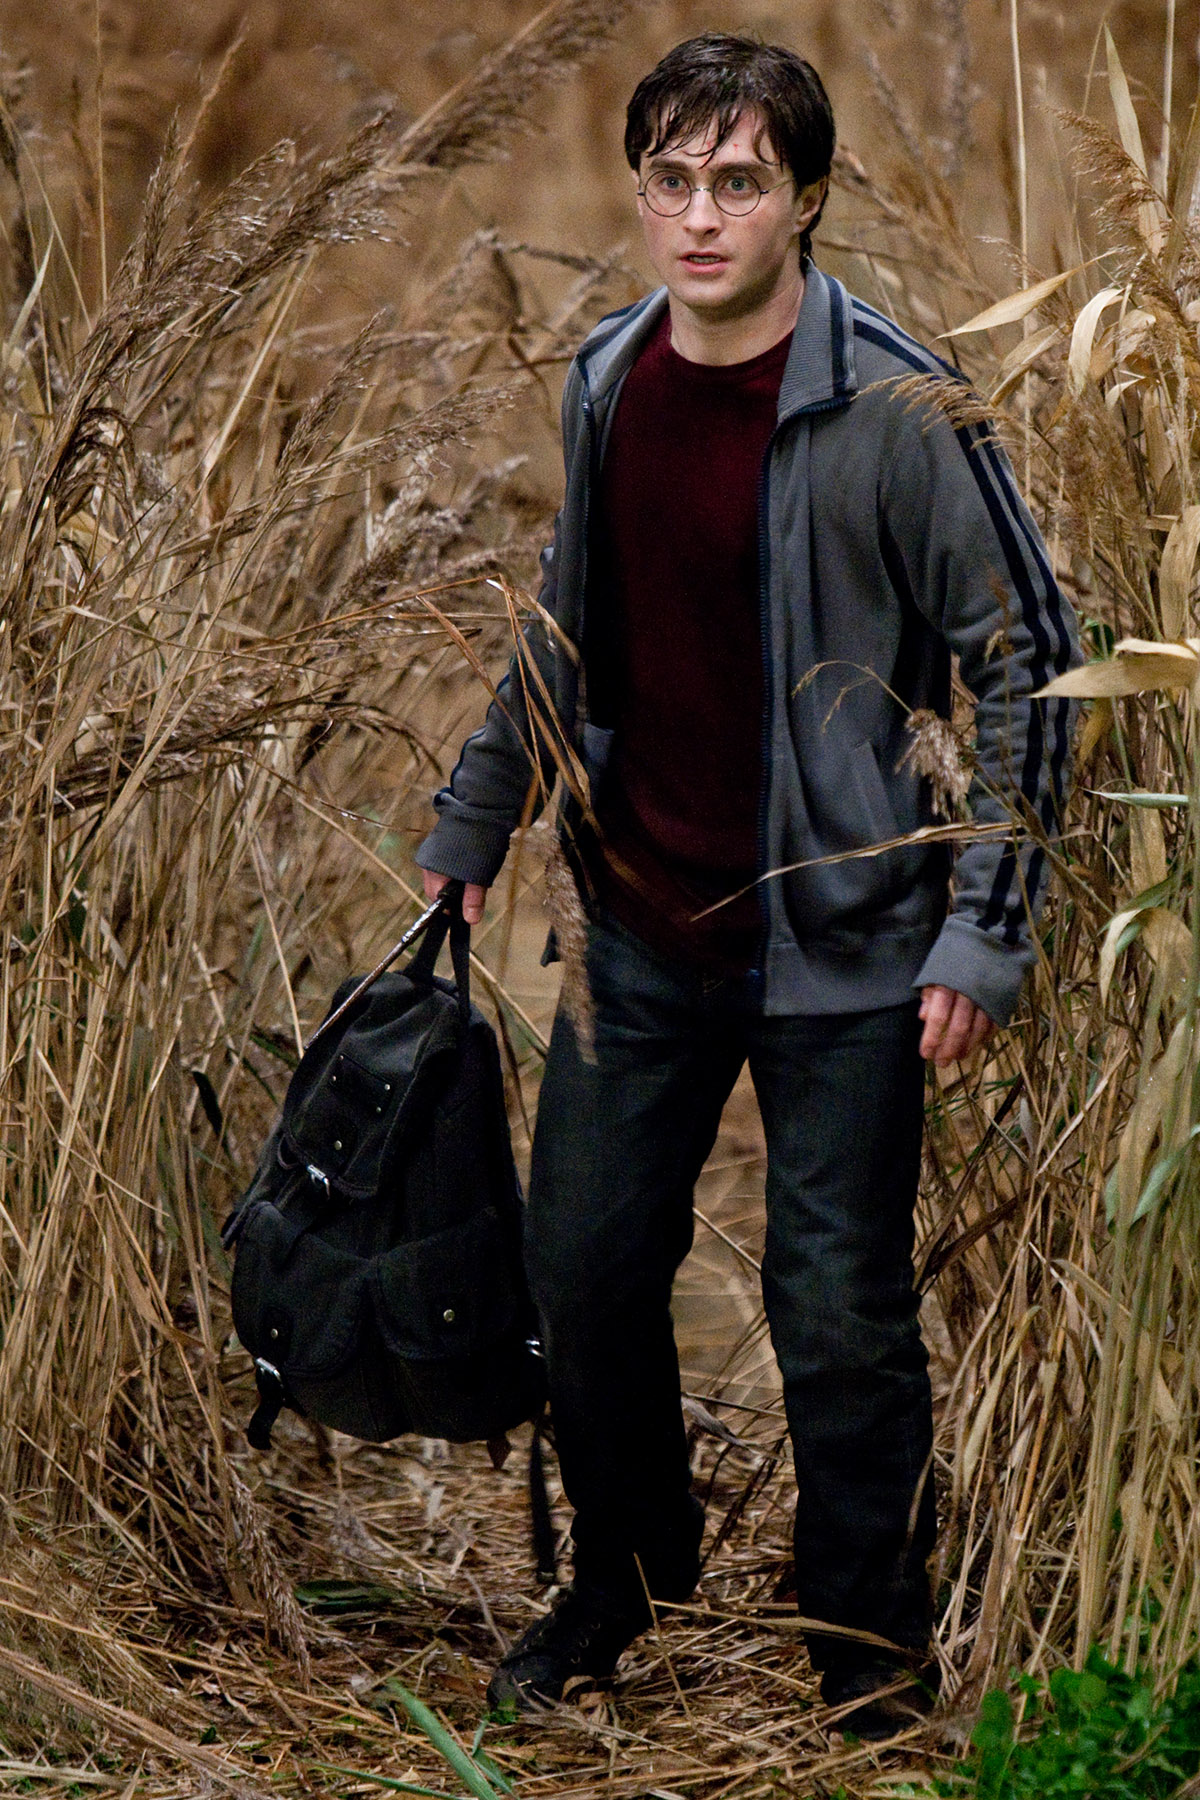
\includegraphics[width=.25\textwidth]{hp.jpg}
  };
	\pause
	\node[inner sep=1mm,align=center] at (3.5,2) {
    
\includegraphics[width=.17\textwidth]{gryffindor.png}
  };
	\pause
	\node[inner sep=1mm,align=center] at (10,2.3) {
    
\includegraphics[width=.25\textwidth]{ron.png}
  };
	\node[inner sep=1mm,align=center] at (10,1) {
    
\includegraphics[width=.15\textwidth]{v.png}
  };
	\pause
	\node[inner sep=1mm,align=center] at (10,-2.3) {
    
\includegraphics[width=.25\textwidth]{draco.png}
  };
	\node[inner sep=1mm,align=center] at (10,-3.6) {
    
\includegraphics[width=.15\textwidth]{x.png}
  };
	\end{tikzpicture}
\end{frame}

\begin{frame}
	\centering
	\begin{tikzpicture}
    \node[inner sep=1mm,align=center] (rust) at (8,0) {
      
\includegraphics[width=.3\textwidth]{rust.png}
    };
    \pause
    \node[inner sep=1mm,align=center]  at (0,-2) {
      
\includegraphics[width=.3\textwidth]{go.png}
    };
    \node[inner sep=1mm,align=center]  at (0.2,1.5) {
      
\includegraphics[width=.3\textwidth]{c.png}
    };
    \draw[->, line width=1mm, color=orange!30] (2.7,0)--(5.2,0);
    \node at (4,0.4){\large DIPPE};
	\end{tikzpicture}

  \begin{center}
    Decentralised ABE scheme, Yan Michalevsky and Marc Joye 2018
  \end{center}
\end{frame}

\section{demo application}

\tikzset{
  planet/.style = {circle, draw=none, fill=blue!30,
    font=\large,
    text width=24mm, inner sep=1mm,align=center}, %<---
  satellite/.style = {circle, draw=none, fill=orange!30,
    text width=18mm, inner sep=1mm, align=center},%<---
}

\begin{frame}
  \begin{columns}
    \begin{column}{.7\textwidth}
      \begin{tikzpicture}
        \node (p)   [planet]  at (0,0)  {server authority};
        \node (s1) [satellite] at (0,-3.5) {client};
        \node (s2) [satellite] at (3,-3.5) {client};
        \node (s3) [satellite] at (-3,-3.5) {client};
        \draw (p)--(s1);
        \draw (p)--(s2);
        \draw (p)--(s3);
      \end{tikzpicture}
    \end{column}
    \begin{column}{.25\textwidth}
      \begin{center}
        
\includegraphics[width=\textwidth]{flickrs.png}

        {\small \url{https://flickrs.opencloudedge.be}}

        
\includegraphics[width=\textwidth]{frame.png}
      \end{center}
    \end{column}
  \end{columns}
\end{frame}

\begin{frame}
  \frametitle{Architecture}
  \begin{columns}
    \begin{column}{.55\textwidth}
      \begin{tikzpicture}
        \node (p)   [planet]  at (0,0)  {server authority};
        \node (s1) [satellite] at (0,-3.5) {client};
        \node (s2) [satellite] at (3,-3.5) {client};
        \node (s3) [satellite] at (-3,-3.5) {client};
        \draw (p)--(s1);
        \draw (p)--(s2);
        \draw (p)--(s3);
      \end{tikzpicture}
    \end{column}
    \begin{column}{.45\textwidth}
      \setbeamersize{description width=2cm}
      \begin{description}
        \item[authority] server on \emph{Kubernetes}
        \item[client] web browser and \emph{WASM}
      \end{description}
    \end{column}
  \end{columns}

  \medskip

  {\small \url{https://flickrs.opencloudedge.be}}
\end{frame}

\begin{frame}
  \frametitle{Architecture}
  \begin{columns}
    \begin{column}{.55\textwidth}
      \begin{tikzpicture}
        \node (p)   [planet]  at (0,0)  {server authority};
        \node (s1) [satellite] at (0,-3.5) {client};
        \node (s2) [satellite] at (3,-3.5) {client};
        \node (s3) [satellite] at (-3,-3.5) {client};
        \draw (p)--(s1);
        \draw[very thick, <->] (p)--(s2);
        \draw (p)--(s3);
      \end{tikzpicture}
    \end{column}
    \begin{column}{.45\textwidth}
      \setbeamersize{description width=2cm}
      \textbf{Setup:}
      \begin{enumerate}
        \item Download webpage and \emph{WASM}
        \item Fetch \emph{authority key}
        \item Request \texttt{UserPrivateKey}
      \end{enumerate}

      \smallskip

      \textbf{Upload} (hybrid encryption):
      \begin{enumerate}
        \item Select \emph{attributes}
        \item Hybrid encryption ChaCha20Poly1305-DIPPE
        \item Upload to server
      \end{enumerate}

      \smallskip

      \textbf{Fetch images:}
      \begin{enumerate}
        \item Fetch \emph{all images}
        \item Hybrid decryption.
      \end{enumerate}
    \end{column}
  \end{columns}

  \medskip

  {\small \url{https://flickrs.opencloudedge.be}}
\end{frame}

\begin{frame}
  \frametitle{preliminary benchmarks}

  \begin{itemize}
    \item In production Kubernetes: ±1\,k user registrations per second on \emph{single machine}\foonote{EPYC Rome 16-core, 64\,GB}.
    \item Encryption with 16 attributes \(k=2\): ±350\,ms\footnote{Threadripper 1920X, 32\,GB}
  \end{itemize}

  \dots future work: compare with CiFEr/GoFE.
\end{frame}

\begin{frame}
  \frametitle{Results \& Caveats}

  We have
  \begin{itemize}
    \item a complete \emph{Rust implementation} with 90\,\%+ test coverage of \emph{DIPPE}
    \item \dots compilable to \emph{WebAssembly}
    \item extensive \emph{documentation} and tested \emph{example code}:\\
      \url{https://etrovub.gitlab.io/smartnets/cife-rs/doc/cife_rs/abe/dippe/index.html}
    \item a live \emph{demo}\footnote{\dots which hopefully didn't fail!}
  \end{itemize}

  \medbreak

  \dots but \dots

  \medbreak

  \begin{itemize}
    \item hash-to-curve is \emph{stubbed} as \texttt{return} \(G\),
      although tested as \texttt{return} \(\mathcal{H}(msg) \cdot G\).
    \item serialization does not use point compression
    \item interop between CiFEr, GoFE and CiFE-rs untested
  \end{itemize}
\end{frame}

\end{document}
